\begin{frame}[label=title]
  \centering
  \begin{figure}[H]
    
\includegraphics[keepaspectratio, width=0.7\paperwidth, height=\paperheight]{LeeLogo}
  \end{figure}
  Informatik: Data Science und Sicherheit\\
  \emoji{floppy-disk} \textbf{\gls{SQL}: mehrere Tabellen}
\end{frame}

\begin{frame}[fragile]{Eine Schul-Datenbank}
  Eine Schule möchte eine Datenbank entwerfen. Sie will folgende Informationen speichern:
  \begin{itemize}
    \item SchülerInnen: Namen, Geschlecht, Geburtsdatum, Wohnort
    \item LehrerInnen: Namen, Geschlecht, Geburtsdatum, Wohnort, Gehalt, Fach (oder Fächer), Klasse (oder Klassen)
    \item Klassen: SchülerInnen, Klassenname, Klassenlehrperson
  \end{itemize}
  Wie viele Tabellen soll die Schule erstellen?
  \only<2->{
    \begin{figure}[H]
      \centering
      \resizebox{\textwidth}{!}{%
        \begin{tikzpicture}
          % Entitäten
          \node[entity] (lehrer) at (0,0) {Lehrer};
          \node[entity] (schueler) at (14,0) {Schüler};
          \node[entity] (klasse) at (7,0) {Klasse};

          % Beziehungen
          \node[relationship] (unterrichtet) at (3.5,0) {unterrichtet};
          \node[relationship] (gehoert_zu) at (10.5,0) {gehört zu};

          % Kanten
          \draw (lehrer) -- (unterrichtet) node[midway,above]{n};
          \draw (unterrichtet) -- (klasse) node[midway,above]{0:1};
          \draw (schueler) -- (gehoert_zu) node[midway,above]{1};
          \draw (gehoert_zu) -- (klasse) node[midway,above]{m};
        \end{tikzpicture}
      }
    \end{figure}
    \begin{myachtung}
      Was bedeuten die Zahlen in der Zeichnung? Stimmen sie?
    \end{myachtung}
  }
\end{frame}

\begin{frame}{Weitere Beispiele}{Es gibt noch viel komplexere Datenbanken...}
  \begin{figure}[H]
    \centering
    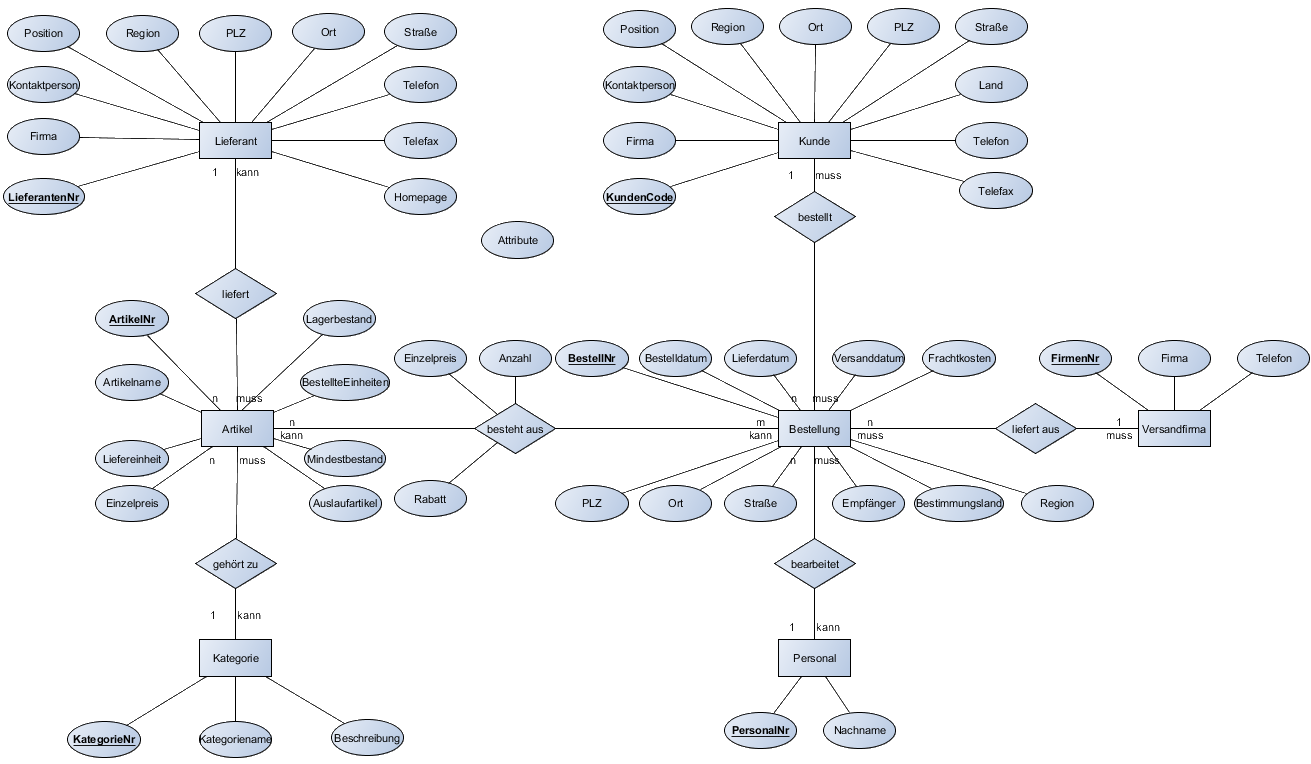
\includegraphics[width=\linewidth]{GrundlagenInfo/DataScience/06_Daten/Figures/er_nordwind_komplett}
    \caption{Datenbank einer Firma, die Produkte verkauft (z.B. Supermarkt)}
  \end{figure}

\end{frame}

\begin{frame}[fragile]{Was ist ein \gls{ERM}?}
  \begin{figure}[H]
    \centering
    \resizebox{\textwidth}{!}{%
      \begin{tikzpicture}[node distance=1cm]

        % Entity
        \node[entity] (entity1) {Entity};
        \node[attribute] (attr1) [above left=of entity1] {Attribute} edge (entity1);
        \node[attribute] (attr2) [below left=of entity1] {Attribute} edge (entity1);

        % Relationship
        \node[relationship] (rel1) [right=3cm of entity1] {Relationship} edge node[auto,swap] {n} (entity1);
        \node[entity] (entity2) [right=3cm of rel1] {Entity} edge node[auto,swap] {m} (rel1);
        \node[attribute] (attr3) [above=of rel1] {Attribute} edge (rel1);

        % Legend
        \node[draw,thick,fit=(entity1) (attr1) (attr2),inner sep=0.5cm, rounded corners, dotted, red] (box1) {};
        \node[anchor=south, red] at (box1.north) {Einheiten (\textit{Entities}) und Attribute};

        \node[draw,thick,fit=(rel1) (entity2) (attr3),inner sep=0.5cm, rounded corners, dotted, blue] (box2) {};
        \node[anchor=south, blue] at (box2.north) {Beziehungen (\textit{Relationships})};

      \end{tikzpicture}}
    \caption{\gls{ERM}-Komponenten in der sogenannten Chen-Notation}
    \label{fig:erm-components}
  \end{figure}
\end{frame}

\begin{frame}[fragile]{\gls{ERM} von InstaHub}
  \begin{figure}[H]
    \centering
    \resizebox{\textwidth}{!}{%
      \begin{tikzpicture}[auto]
        % Nodes
        \node[entity] (user) at (0,0) {users};
        \node[relationship] (follows) at (-4,0) {follows};
        \node[relationship] (owns) at (2.5,2.5) {owns};
        \node[entity] (photo) at (5,0) {photos};
        \node[relationship] (has) at (7,0) {has};ff
        \node[entity] (tag) at (9,0) {tags};
        \node[relationship] (comments) at (2.5,0) {comments};
        \node[relationship] (likes) at (2.5,-2.5) {likes};
        \node[relationship] (haspw) at (0,-2) {has};
        \node[entity] (pwreset) at (-4,-2) {password\_resets};

        % Edges
        \draw (user) -- (follows) node[midway, above] {m};
        \draw (follows) -- (user) node[midway, below] {n};
        \draw (user) -- (owns) node[midway, above] {1};
        \draw (owns) -- (photo) node[midway, above] {n};
        \draw (photo) -- (has) node[midway, above] {n};
        \draw (has) -- (tag) node[midway, above] {m};
        \draw (user) -- (comments) node[midway, above] {n};
        \draw (comments) -- (photo) node[midway, above] {m};
        \draw (user) -- (likes) node[midway, left] {n};
        \draw (likes) -- (photo) node[midway, right] {m};
        \draw (user) -- (haspw) node[midway, left] {1};
        \draw (haspw) -- (pwreset) node[midway, above] {n};
      \end{tikzpicture}}
    \caption{\gls{ERM} von InstaHub (ohne Attribute)}
    \label{fig:erm-instahub}
  \end{figure}
  \only<2->{
    \textbf{Kardinalität} einer Beziehung
    \begin{itemize}
      \item Eins-zu-Eins (1:1)
      \item Eins-zu-Viele (1:n)
      \item Viele-zu-Viele (m:n)
    \end{itemize}
  }
\end{frame}

\begin{frame}[fragile]{\lstinline[style=sql]|JOIN|-Typen}
  \begin{figure}[htbp]
    \centering

    % INNER JOIN
    \begin{subfigure}[b]{0.45\textwidth}
      \centering
      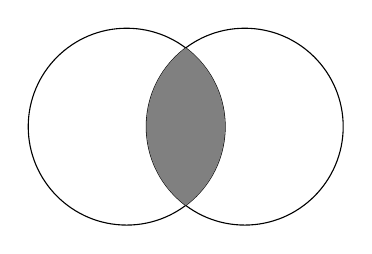
\begin{tikzpicture}
        \tikzset{circle node/.style={circle,draw=black, fill=none, minimum size=25mm, inner sep=0pt}}
        \node[circle node] (left) at (0,0) {};
        \node[circle node] (right) at (1.5,0) {};
        \begin{scope}
          \clip (0,0) circle (1.25cm);
          \fill[gray] (1.5,0) circle (1.25cm);
        \end{scope}
      \end{tikzpicture}
      \caption{\lstinline[style=sql]|INNER JOIN|}
    \end{subfigure}
    \hfill
    % LEFT OUTER JOIN
    \begin{subfigure}[b]{0.45\textwidth}
      \centering
      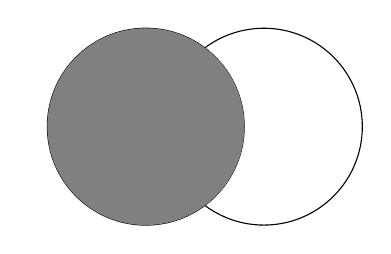
\begin{tikzpicture}
        \tikzset{circle node/.style={circle,draw=black, fill=none, minimum size=25mm, inner sep=0pt}}
        \node[circle node] (left) at (0,0) {};
        \node[circle node] (right) at (1.5,0) {};
        \begin{scope}
          \clip (-1.5,-1.25) rectangle (1.25,1.25);
          \fill[gray] (0,0) circle (1.25cm);
        \end{scope}
        \begin{scope}
          \clip (0,0) circle (1.25cm);
          \fill[gray] (1.5,0) circle (1.25cm);
        \end{scope}
      \end{tikzpicture}
      \caption{\lstinline[style=sql]|LEFT OUTER JOIN|}
    \end{subfigure}

    \bigskip

    % RIGHT OUTER JOIN
    \begin{subfigure}[b]{0.45\textwidth}
      \centering
      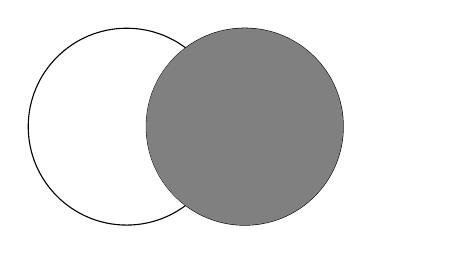
\begin{tikzpicture}
        \tikzset{circle node/.style={circle,draw=black, fill=none, minimum size=25mm, inner sep=0pt}}
        \node[circle node] (left) at (0,0) {};
        \node[circle node] (right) at (1.5,0) {};
        \begin{scope}
          \clip (0,-1.25) rectangle (4,1.25);
          \fill[gray] (1.5,0) circle (1.25cm);
        \end{scope}
        \begin{scope}
          \clip (1.5,0) circle (1.25cm);
          \fill[gray] (0,0) circle (1.25cm);
        \end{scope}
      \end{tikzpicture}
      \caption{\lstinline[style=sql]|RIGHT OUTER JOIN|}
    \end{subfigure}
    \hfill
    % FULL OUTER JOIN
    \begin{subfigure}[b]{0.45\textwidth}
      \centering
      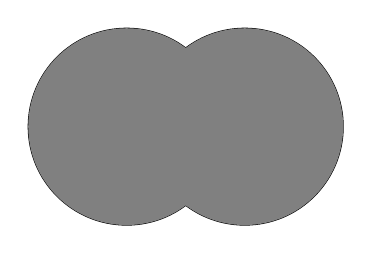
\begin{tikzpicture}
        \tikzset{circle node/.style={circle,draw=black, fill=none, minimum size=25mm, inner sep=0pt}}
        \node[circle node] (left) at (0,0) {};
        \node[circle node] (right) at (1.5,0) {};
        \fill[gray] (0,0) circle (1.25cm);
        \fill[gray] (1.5,0) circle (1.25cm);
      \end{tikzpicture}
      \caption{\lstinline[style=sql]|FULL OUTER JOIN|}
    \end{subfigure}
    \caption{Venn-Diagramme unterschiedlicher SQL-Joins}
    \label{fig:venn-joins}
  \end{figure}
\end{frame}

\begin{frame}[fragile]
  \begin{center}
    Demo: InstaHub
  \end{center}
\end{frame}

\begin{frame}[fragile]{Aufgaben}
  Skript (Moodle)
  \begin{itemize}
    \item \aufgabebox{Aufgabe 2.47}
    \item Aufgaben und Abgaben in Kapiteln 2.3 und 2.4
  \end{itemize}
\end{frame}